\section{Виды ошибок}\label{5000}
\subsection{Сумма по эквайрингу больше суммы б/н в Z-отчете}
%\marginnote{\Date{Чт.}{19}{Июл.}{2018}}[-40pt]

\begin{itemize}	
	\item Ситуация возникает, когда при проведении платежа, обмен с банком и списание денег с карты клиента происходит, а чек через фискальный регистратор не пробивается.
	
	
	\begin{myquote}
		Подобная ситуация когда чек по эквайрингу прошел, а по фискальнику нет, должна штатно решаться в реальном времени кассиром, который снимает х-отчеты для того что бы убедиться, что оплата по банку прошла и делает текущий чек «отложенным» и затем проводит и пробивает его согласно «инструкции для кассиров п2.1.
	\end{myquote}
	
	
	\begin{figure}[H]
		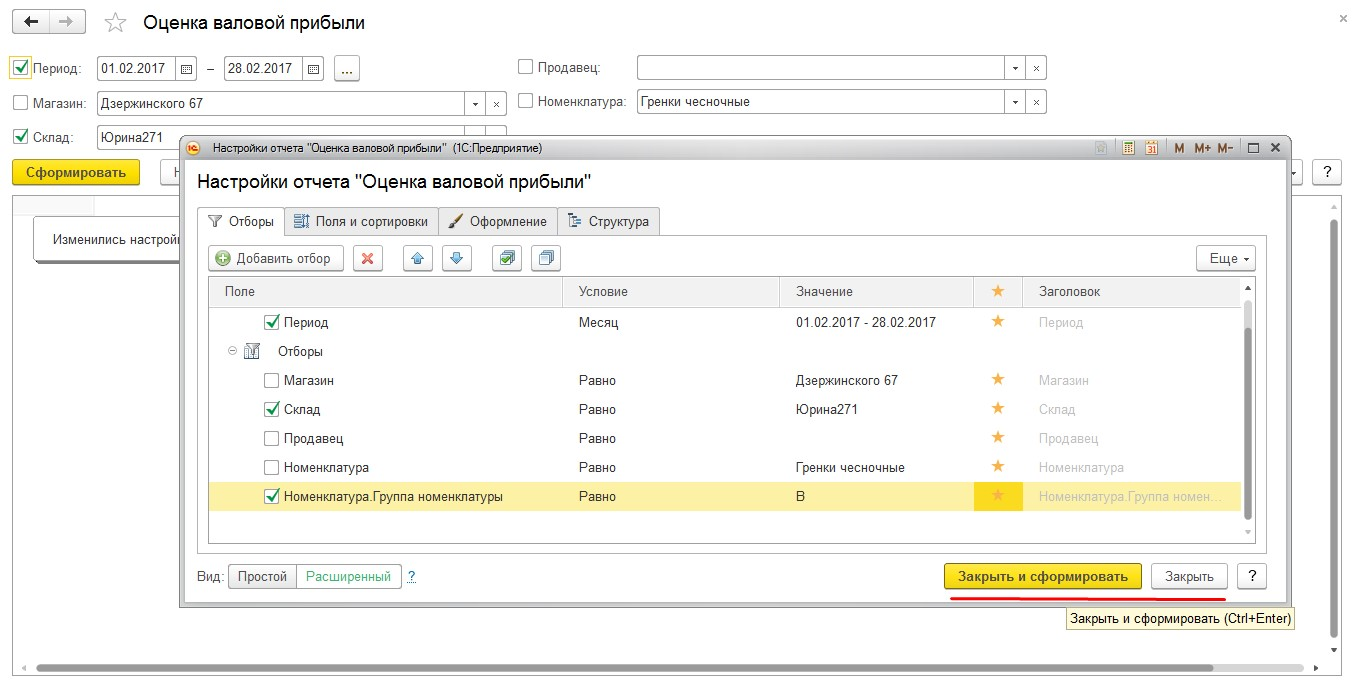
\includegraphics[width=1.0\textwidth]{11.jpg}
		\caption{<<Эквайринг>>.}
		\label{ris:11.jpg}
	\end{figure}
	Здесь видно, что сумма по эквайрингу на 100 р. больше суммы по безналу.  (Рис.~\ref{ris:11.jpg})
	\item Первое, что необходимо сделать - проверить по бумажным отчетам, что суммы внесены правильно. И если это действительно так и есть расхождения сумм  в слип чеке и Z- отчете, а не допущена ошибка ввода, приступаем к поискам потерянного чека. Нужно путем опроса кассиров выяснить, какой товар был в этом чеке.
    
 %   \todo{Что делать если содержимое чека не удалось восстановить}\par
    
	Установив товар в чеке или приняв решение чем его заменить нам нужно добавить этот чек в текущем дне, когда мы исправляем ошибки. Есть два способа это сделать:	
	
	\begin{enumerate}[label={\Alph*)},font={\color{blue!50!black}\bfseries}] 
		\item Если смена на кассе ОТКРЫТА Создать чек сегодняшним днем с видом оплаты «оплата картой», по нужной кассе (на компьютере  товароведа), записать его НЕ ПРОВОДЯ!  Далее, УЖЕ НА КАССЕ пробить его по фискальнику как отложенный чек (нажав кнопку \keys{ВЫПОЛНИТЬ}).
%  \footnote {Либо переписть обработку по работе с чеками и упростить ее для товароведов. }\par		
		
		\item Если смена на кассе еще НЕ ОТКРЫТА, то открыть смену, создать чек НА КАССЕ. Поместить этот чек в «отложенные». пробить его по фискальнику как отложенный чек (нажав кнопку \keys{ВЫПОЛНИТЬ}) и  смену закрыть.
%  \footnote {Сейчас при ручном создании ОРП не создается запись в регистре <<Опрос кассиров по окончании смены>> и ОРП не проводится, нужно решить этот вопрос }\par
	\end{enumerate}

%This is text \raisebox{1em}{\makebox[1pt]{\tiny Hint text}}with primechaniya.


	
%	\todo{Расписать работы с актом списания}\par
	
\end{itemize}
